\documentclass{beamer}

\usepackage{amsmath,amssymb,graphicx}
\usepackage{tikz}
\usetikzlibrary{positioning,shapes.geometric,decorations.text}

\usetheme{default}
\usecolortheme{wolverine}

\newcommand{\E}{\mathbb{E}}
\newcommand{\indp}{\ensuremath{\perp\hspace{-5pt}\perp}}
\newcommand{\M}{\mathcal{M}}
\newcommand{\given}{\; \mid \;}
\DeclareMathOperator{\logit}{logit}

\title[Project Presentation]{ The effect of ``attempting to lose weight'' on sleep }
\author{Alex Luedtke, Lucia Petito, Steven Pollack}
\institute{PHC252D}
\date{}

\begin{document}
\maketitle 
\begin{frame}
 \frametitle{Roadmap} 
  \begin{itemize}
    \item Background
    \item Specify SCM (and DAG)
    \item Specify counterfactuals and target causal quantity
    \item Introduce data and commit to a statistical model
    \item Discuss identifiability and estimand
    \item Get our hands dirty (estimation procedures)
    \item Results
    \item Interpretation
  \end{itemize}
\end{frame}

\begin{frame}
 \frametitle{Background}
 We know that sleep habits affect weight, but does trying to lose weight affect sleep patterns?
  \begin{itemize}
    \item Doctors advise consistently getting enough sleep each night to maintain a healthy lifestyle.  
    \item Previous research has shown an association between sleep deprivation and obesity and oversleeping and obesity (indicates a U-shaped curve).
    \item Hormonal changes from dieting could cause disruptions in sleep cycle (could also be caused by exercise).
  \end{itemize}
\end{frame}

\begin{frame}
 \begin{itemize}
  \item We used National Health and Nutrition Examination Survey (NHANES) data -- from the National Center for Health Statistics (NCHS) -- a multistage survey of U.S. population
 \end{itemize}
 \begin{figure}
 \centering
  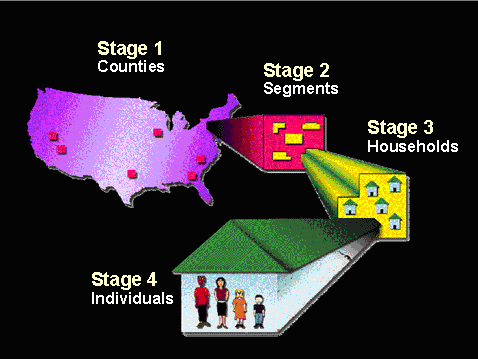
\includegraphics[width=0.5\textwidth]{Survey_Design.PNG}
  \caption{Picture courtesy of NHANES}
 \end{figure}
 \begin{itemize}
  \item Survey aims to study wide range of topics such as Cardiovascular disease, Obesity, Physical fitness and physical functioning, Reproductive history and sexual behavior, etc.
 \end{itemize}
\end{frame}

\begin{frame}
  \frametitle{Background (Cont'd)}
  Notes about NHANES data:
  \begin{itemize}
 \item Individuals were subjected to interviews as well as physical examinations.
  \begin{itemize}
    \item categorical as well as numerical data
    \item some questions had a lot of valid responses, but made practical positivity questionable.
    \item No shortage of missing data (either ``I don't know''s or unanswered questions).
  \end{itemize}
 \item The sample for the survey is selected to represent the U.S. population of all ages. To produce reliable statistics, NHANES over-samples persons 60 and older, adolescents, African Americans, and Hispanics.
 \end{itemize}
\end{frame}

\begin{frame}
\frametitle{$W$: Baseline Covariates}
   \begin{itemize}
   \item When interview was conducted (November 1, 2009 - April 30, 2010 or May 1, 2010 - October 31, 2010)
   \item Gender
   \item Age in months (300-959 months, 25-79 years)
   \item Race/Ethnicity (Mexican American, Other Hispanic, Non-Hispanic White, Non-Hispanic Black, Other)
   \item Education Level (less than high school, high school/GED, some college, college and above)
   \item Marital Status (never married, married/living with partner, divorced/separated)
   \item Annual Household Income (less than or greater than \$20k)
   \item Body Mass Index from one year ago (continuous from 15-50)
  \end{itemize}
\end{frame}

\begin{frame}
 \frametitle{$A$: Exposure Variable}
  \begin{itemize}
    \item The subject's response to the question: ``During the past 12 months, have you tried to lose weight?"
    \item Note that this does not restrict to dieting
  \end{itemize}
\end{frame}

\begin{frame}
 \frametitle{$Y$: Response Variable}
  \begin{itemize}
    \item The subject's response to the question: ``How much sleep do you usually get at night on weekdays or workdays?
    \item Both $A$ and $Y$ sampled simultaneously, so temporal ordering is only assumed
  \end{itemize}
\end{frame}

\begin{frame}
\frametitle{Massaging the Data}
  \begin{itemize}
    \vfill \item Deleted all people who refused to identify Race/Ethnicity, Education Level, Marital Status, Annual Household Income, dieting status
    \vfill \item Forced to coarsen the categories in Annual Household Income
    \vfill \item Collapsed Marital Status to Married/Living with a domestic partner vs. everything else
    \vfill \item Modified Education Level to 1) less than a high school diploma, 2) high school diploma/GED, 3) some college, and 4) college diploma or more
  \end{itemize}
\end{frame}

\begin{frame}
\frametitle{SCM and DAG}

\begin{minipage}{0.55\linewidth}
Our observational data structure is $O=(W,A,Y) \sim P_0$. With mild temporal assumptions, one SCM is:
\begin{align*}
W &= f_{W}(U_{W}) \\
A &= f_{A}(W,U_{A}) \\
Y &= f_{Y}(W,A,U_{Y}) \\
\end{align*}
Note: no assumptions made on functional forms of $W$, $A$, or $Y$.
\end{minipage}
\begin{minipage}{0.4\linewidth}
  \begin{figure}[h]
    \centering
    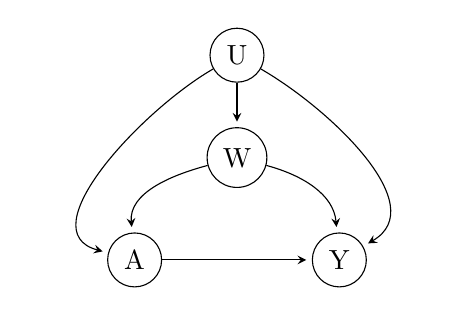
\begin{tikzpicture}[->, shorten >=2pt, >=stealth, node distance=1cm,
                        pil/.style={->,thick,shorten =2pt,},scale=0.65
                        ]
    \node[circle,draw] at (4,2) (1) {W};
    \node[circle,draw] at (2,0) (2) {A};
    \node[circle,draw] at (6,0) (3) {Y};
    \node[circle,draw] at (4,4) (4) {U};
    \draw[->] (1) to [out=195,in=95] (2);
    \draw[->] (2.east) -- (3.west);
    \draw[->] (1) to [out=345,in=95] (3);
    \draw[->] (4.south) -- (1.north);
    \draw[->] (4) to [out=210,in=165] (2);
    \draw[->] (4) to [out=330,in=30] (3);
    \end{tikzpicture}
  \caption{Simplified DAG -- no independence assumptions on $U$'s.}
  \label{fig:DAG}
  \end{figure}
\end{minipage}
\end{frame}

\begin{frame}
 \frametitle{Counterfactuals and Causal Quantities\ldots}
  \begin{itemize}
    \item  Since the intervention is a point treatment, our counterfactual is $Y_{a}$: the average sleep one would get, if they, possibly contrary to fact, had (or had not) attempted to lose weight.
    \item[]
    \item  We are interested in measuring the ATE of attempted weight lose on average sleep:
    \[
      \Psi(P_{U,X}) = \E_{U,X}[Y_1] - \E_{U,X}[Y_0]
    \]
  \end{itemize}
 \end{frame}

\begin{frame}
 \frametitle{Identifiability}
\begin{minipage}{0.45\linewidth}
 \begin{itemize}
   \item Since $\Psi$ is the ATE, we need to satisfy backdoor criterion to identify g-computation with $\Psi$:
   \[
   Y_{a} \indp A \mid W
   \]
   \item Need $U_{A} \indp U_{Y}$ and either
    \begin{itemize}
      \item $U_{A} \indp U_{W}$  (semi-plausible)
      \item $U_{W} \indp U_{Y}$  (less plausible)
    \end{itemize}
 \end{itemize}
\end{minipage}
\begin{minipage}{0.45\linewidth}
    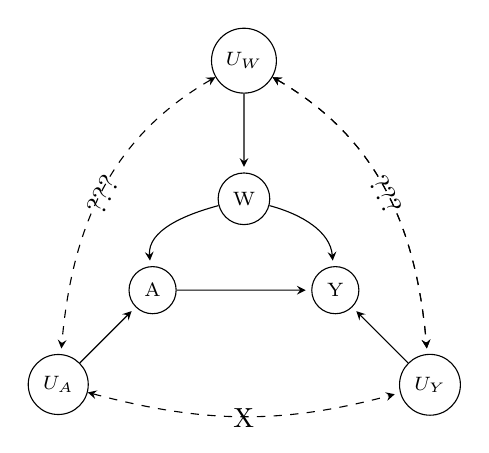
\begin{tikzpicture}[->, shorten >=2pt, >=stealth, node distance=1cm,
                        pil/.style={->,thick,shorten =2pt,},scale=0.65,font=\scriptsize
                        ]
    \node (A) [circle,draw] {A};
    \node (W) [circle,draw,above right=of A] {W};
    \node (Y) [circle,draw,below right=of W] {Y};
    \node (UA) [circle,draw,below left=of A] {$U_A$};
    \node (UW) [circle,draw,above=of W] {$U_W$};
    \node (UY) [circle,draw,below right=of Y] {$U_Y$};
    \draw[->] (W) to [out=195,in=95] (A);
    \draw[->] (A.east) -- (Y.west);
    \draw[->] (W) to [out=345,in=95] (Y);
    \draw[->] (UW.south) -- (W.north);
    \draw[->] (UA) to [out=45,in=225] (A);
    \draw[->] (UY) to [out=135,in=315] (Y);
    \draw[dashed,<->] (UW) to [out=330,in=95] (UY);
    %\pgftransformyshift{-.65cm}
    %\draw[decoration={text along path, text={X},text align={center}},decorate] (UA) to
                      [out=345,in=195] (UY);
    \draw[dashed,<->,postaction={decorate,decoration={raise=-4pt,text along path,text align=center,text={X}}}] (UA) to [out=345,in=195] (UY);
    \draw[dashed,<->,postaction={decorate,decoration={raise=-4pt,reverse path,text along path,text align=center,text={???}}}] (UW) to [out=210,in=85] (UA);
    \draw[dashed,<->,
    postaction={decorate,
    decoration={raise=-4pt,text along path,text align=center,text={???}}}] (UW) to [out=330,in=95] (UY);
    \end{tikzpicture}
\end{minipage}
\end{frame}

\begin{frame}
 \frametitle{Statistical Models}
 \begin{itemize}
  \item No assumptions on the functional forms of $f_W, f_A, f_Y$.
  \item Choose the (non-parametric) model, $\M$, of distributions compatible with our SCM.
 \end{itemize}
\end{frame}

\begin{frame}
\frametitle{Positivity Concerns}
\begin{itemize}
 \item We do not believe that trying to lose weight or not trying to lose weight occurs with probability $0$ given any set of  covariates $W$
 \item Practical positivity violations are a concern given $W$ is high dimensional
\end{itemize}
\end{frame}

\begin{frame}
\frametitle{Results (Cont'd)}
\begin{itemize}
 \item Practical positivity violations for now only assessed on categorical variables $V\subset W$
 \begin{itemize}
  \item Gender, Race/ethnicity, Education Level, Marital Status
 \end{itemize}
 \item No members in our sample who tried to lose weight given:
\end{itemize}
\begin{tabular}{| l | l | l | l |}
\hline
 Gender & Race & Education & Marital Status \\
\hline
Male & Other & Less than HS & Unmarried/not living with partner \\
Female & Other & HS & Married/living with partner \\
\hline
\end{tabular}
\end{frame}

\begin{frame}
\frametitle{Estimands}
Provided we can accept $U_A \indp U_W$ or $U_W \indp U_Y$, we have:
\begin{itemize}
  \item Simple Substitution:
    \[
      \psi_0 \approx \frac{1}{n}\sum_{i=1}^{n}\widehat{\E}\left[Y \mid A=1, W=W_i \right] - \widehat{\E}\left[Y \mid A=0, W=W_i\right]
    \]
  \item IPTW:
  \[
    \psi_{0} \approx \frac{1}{n}\sum_{i=1}^{n} \left(\frac{I(A_i=1)}{\hat{g}_n(A_i \mid W_i)} - \frac{I(A_i=0)}{\hat{g}_n(A_i \mid W_i)} \right)Y_i
  \]
  \item TMLE:
  \[
    \psi_{0} \approx \frac{1}{n}\sum_{i=1}^{n}\left( \bar{Q}_{n}^{1}(1,W_i) - \bar{Q}_{n}^{1}(0,W_i)\right)
  \]
%   where
%   \[
%   \bar{Q}_{n}^{1}(A,W) = \logit(\bar{Q}_{n}^{0}(A,W)) + \epsilon_{n}\left(\frac{I(A=1)}{\hat{g}_n(A=1\mid W)} - \frac{I(A=0)}{\hat{g}_n(A=0\mid W)} \right)
%   \]
\end{itemize}
\end{frame}

\begin{frame}
\frametitle{Estimation Procedures}
Estimate $\bar{Q}_{n}^{0}(a,w) = \widehat{\E}(Y \mid A=a, W=w)$ (and $\hat{g}_{n}(a\mid w)$) via Super Learner with library:
\begin{table}[ht!]
\begin{tabular}{ll}
SL.mean & $Y \sim A$ \\
SL.earth & $Y \sim A \times Gender \times RaceEth + MarStat \times HHInc$ \\
SL.rpartPrune & $+ AgeMonths$:$Gender + EduLevel + AgeMonths $ \\
SL.ridge & $Y \sim A \times Gender \times MarStat$ \\
SL.glmnet &  $Y \sim A \times Gender \times AgeMonths \times HHInc$ \\
\end{tabular}
\caption{Super Learner library}
\end{table}
%Is the : a typo? And we'll estimate the treatment mechanism using the same library and glm's but without regressing on $A$.
\end{frame}

\begin{frame}
\frametitle{Preliminary Results}
\begin{itemize}
\item Multistage survery design makes bootstraping more involved than usually the case.
\item Individuals have survey weights associated to them, however we're unsure how to incorporate these weights during analysis
\item High dimensionality of $W$ makes assessing positivity difficult.
\item The following analysis was performed using ``simple random sampling'' procedure during the bootstrap and equal weighting for individuals.
\end{itemize}
\end{frame}

\begin{frame}
\frametitle{Results (Cont'd)}
\begin{figure}
\centering
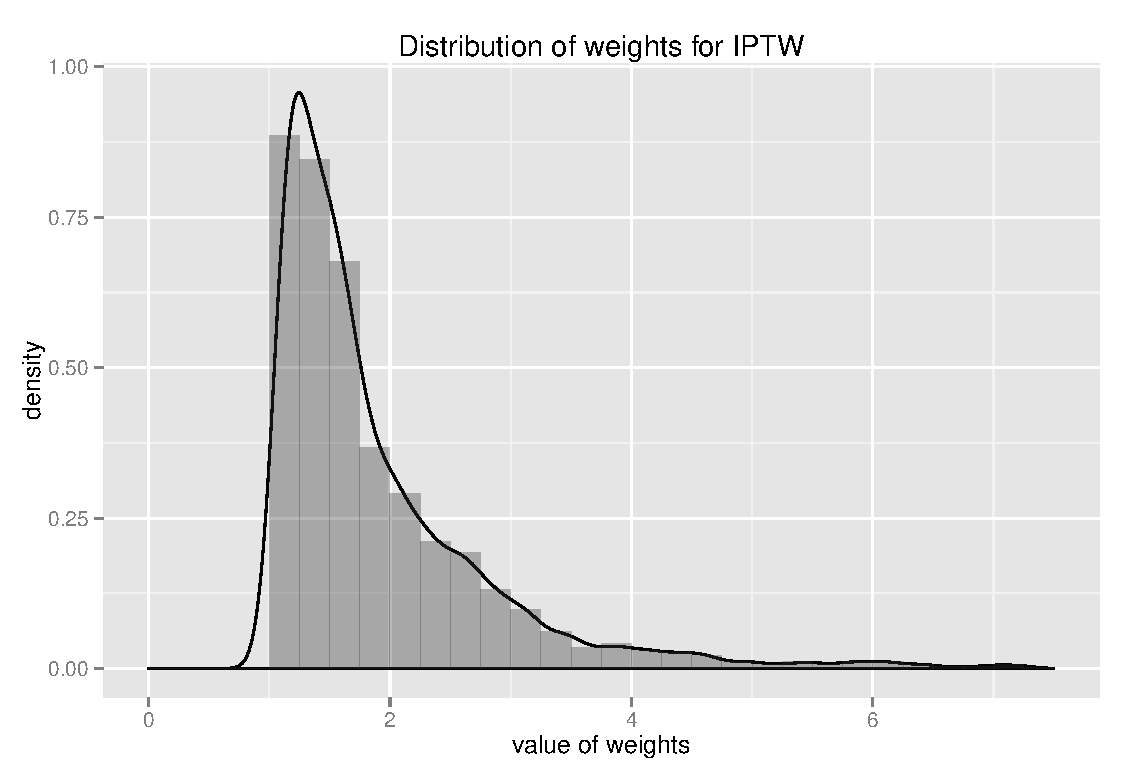
\includegraphics[width=0.75\textwidth]{density-plot_ghat.pdf}
\caption{Histogram and Density estimate of weights from SuperLearner output of $g_n$.}
\end{figure}
\end{frame}

\begin{frame}
\frametitle{Results (Cont'd)}
Most of the mass of the weights in $(0,7.5)$, but \texttt{weights} takes on value over 25 once.
\begin{table}[ht]
\centering
\begin{tabular}{cccccc}
  \hline
 Min. & 25\% & Median & Mean & 75\% & Max. \\ 
  \hline
 1.037   & 1.281   & 1.587   & 1.952   &  2.198   &  35.335   \\ 
   \hline
\end{tabular}
\caption{Summary of distribution of weights}
\end{table}
\end{frame}

\begin{frame}
\frametitle{Results (Cont'd)}
\begin{figure}
\centering
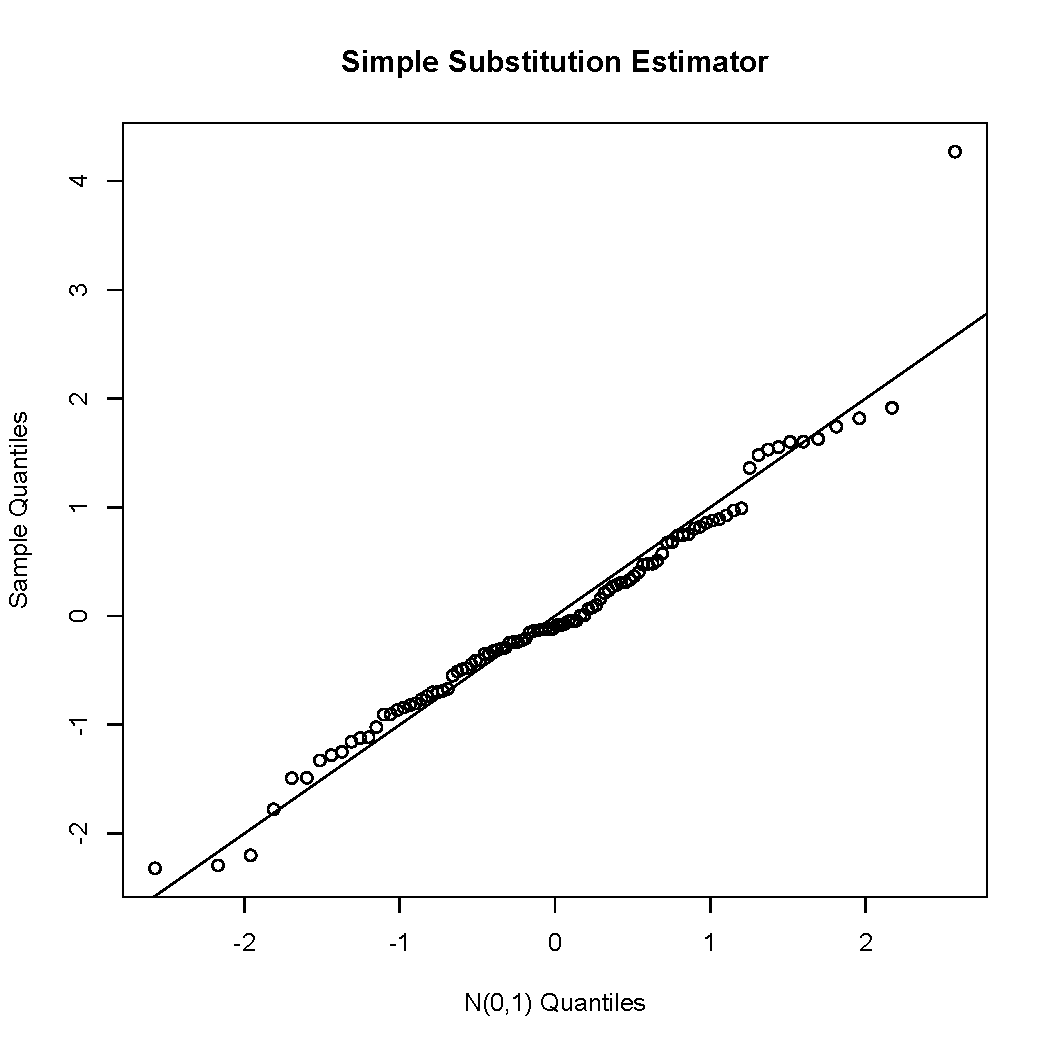
\includegraphics[width=0.45\textwidth]{simplesub_qqplot.pdf}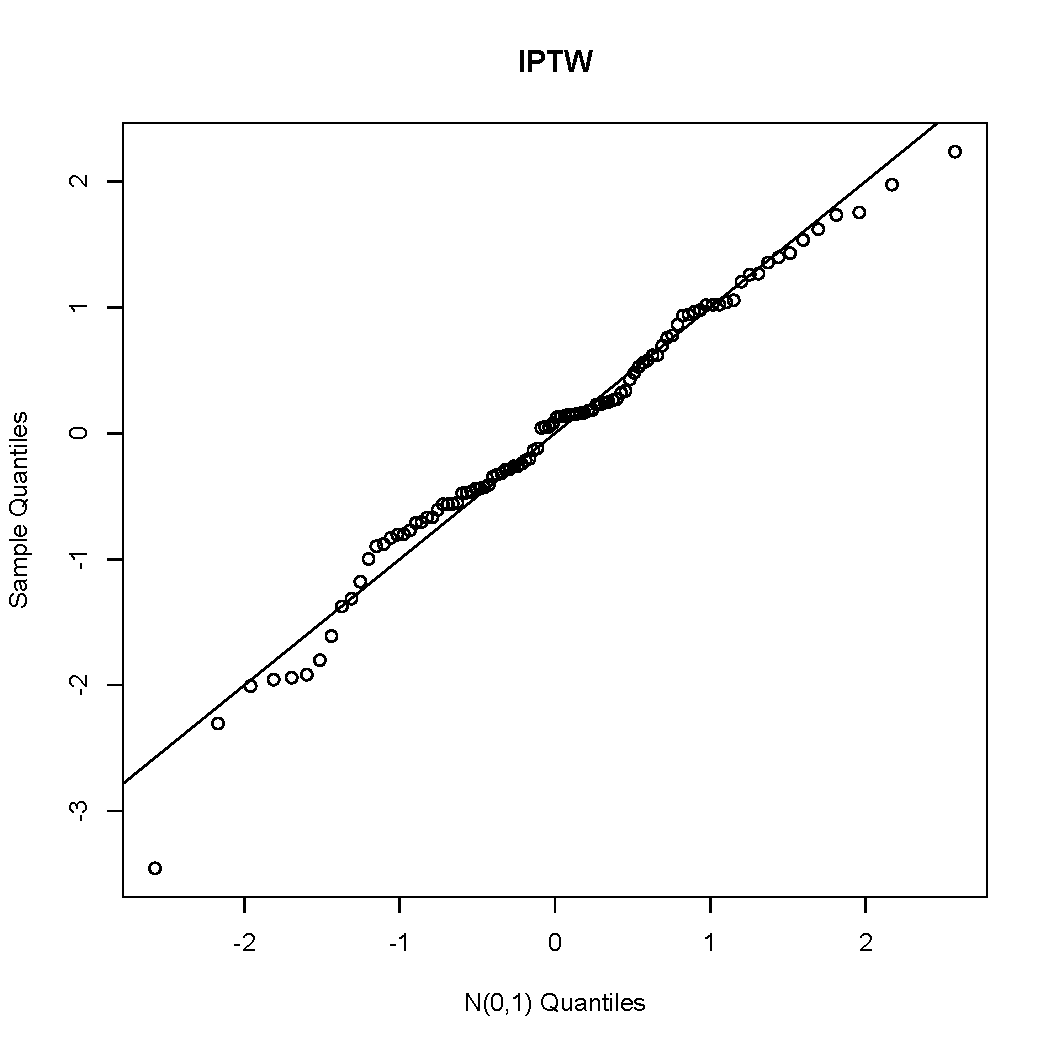
\includegraphics[width=0.45\textwidth]{iptw_qqplot.pdf}
\caption{Q-Q plots for G-Comp and IPTW estimators against Normal}
\end{figure}
\end{frame}

\begin{frame}
\frametitle{Results}
\begin{figure}
\centering
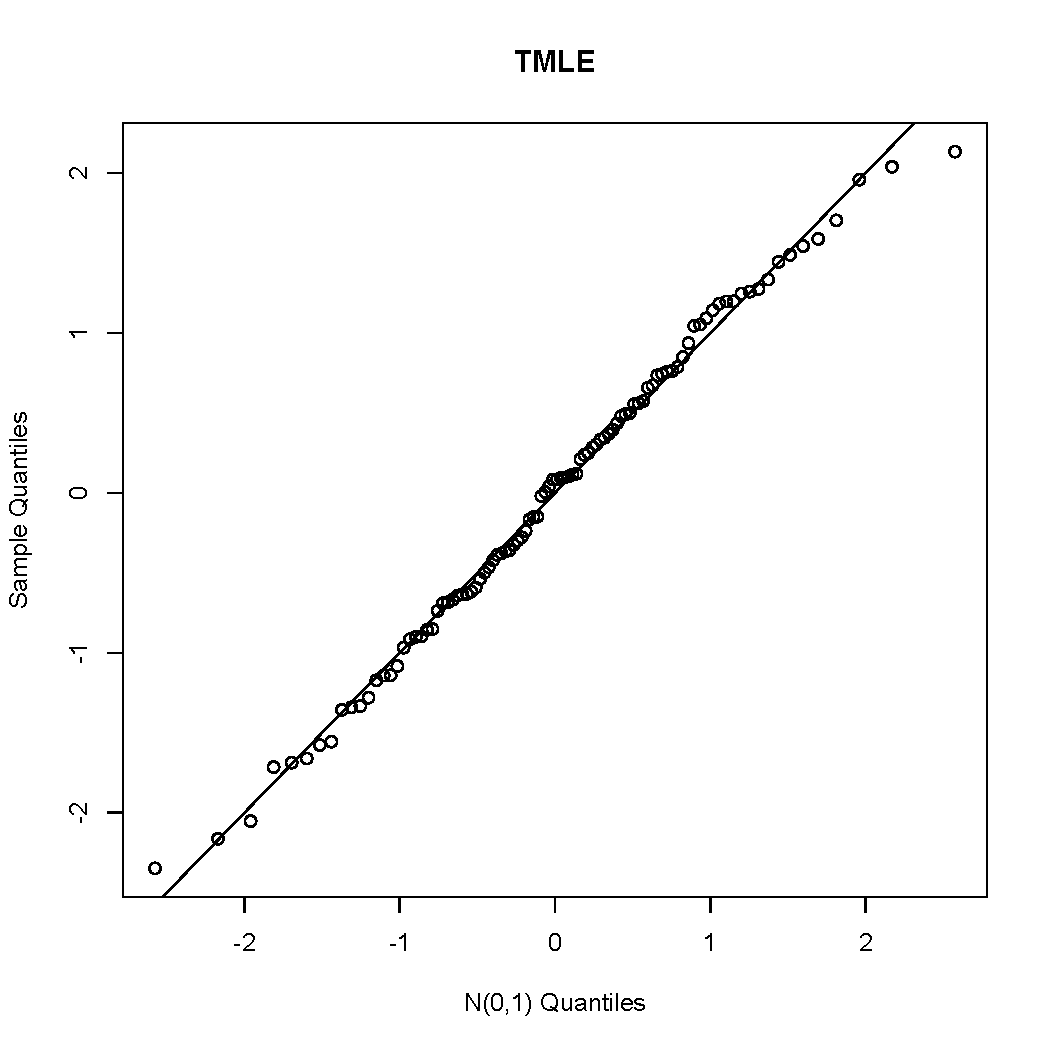
\includegraphics[width=0.75\textwidth]{tmle_qqplot.pdf}
\caption{Q-Q plot for TMLE sampling distribution against Normal}
\end{figure}
\end{frame}

\begin{frame}
\frametitle{Results (Cont'd)}
\begin{figure}[ht!]
\centering
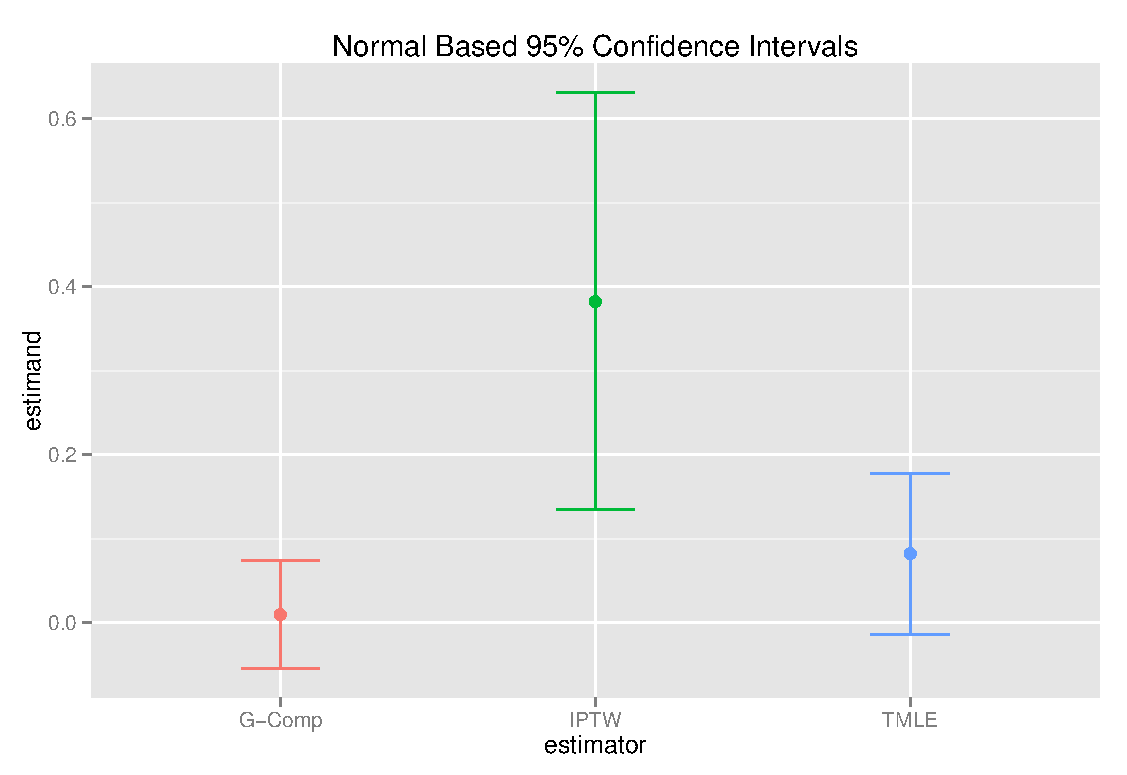
\includegraphics[width=0.75\textwidth]{bootstrap-normal-ci.pdf}
\caption{95\% Confidence intervals based on Normal approximation\ldots}
\end{figure}
\end{frame}

\begin{frame}
\frametitle{Results (Cont'd)}
\begin{table}[ht]
\centering
{\small
\begin{tabular}{rcccc}
  \hline
 & Estimate & 95\% Normal CI & 95\% Quantile CI \\ 
  \hline
G-Comp & 0.00983 & (-0.05444, 0.07411) & (-0.04403, 0.07961) \\ 
  IPTW & 0.38282 & (0.13473, 0.63091) & (0.40209, 0.89568) \\ 
  TMLE & 0.08175 & (-0.01418, 0.17769) & (-0.01667, 0.16519) \\ 
   \hline
\end{tabular}
}
\caption{Results for na\"{i}ve small sample bootstrap}
\end{table}
\end{frame}

\begin{frame}
\frametitle{Results (Cont'd)}
\begin{figure}[ht!]
\centering
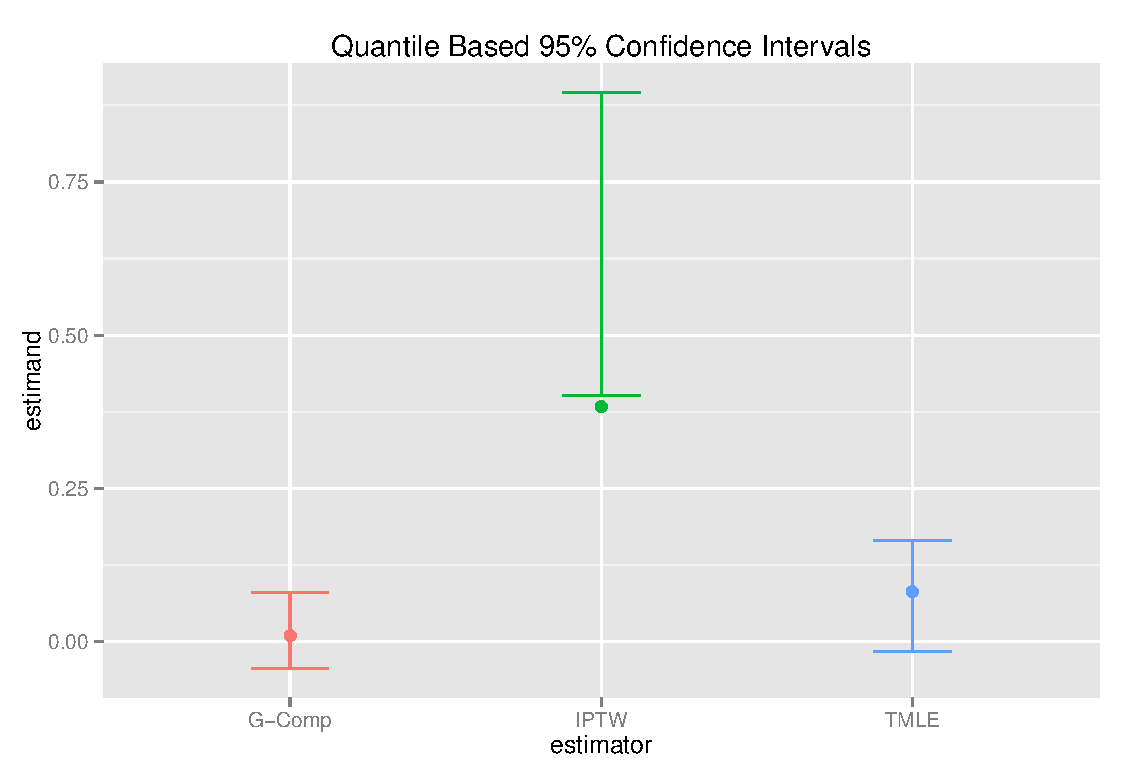
\includegraphics[width=0.75\textwidth]{bootstrap-quantile-ci.pdf}
\caption{95\% Confidence intervals based off of Bootstrap Quantiles\ldots}
\end{figure}
\end{frame}

\begin{frame}
\frametitle{Shortcomings}
  \begin{itemize}
    \vfill\item Removed all missing data on a complete-case basis: deleted 2,832 people
    \vfill\item Should have more covariates (tv watching, prescription medicines, etc)
    \vfill\item Impossible to accurately bootstrap as it stands: did not account for survey weights
    \vfill\item Did not account for survey weights in our GLMs
    \vfill\item Difficult temporal ordering
    \vfill\item Identifiability implausible ($U_W$ probably not independent of $U_Y$)
    \vfill\item Covariates do not have predictive power for $Y$: SuperLearner performs similarly to basic GLM
  \end{itemize}
  \vfill
\end{frame}
\end{document}